\documentclass[10pt,conference,compsocconf]{IEEEtran}

\usepackage{hyperref}
\usepackage{graphicx}	% For figure environment


\begin{document}
\title{Machine Learning - Project 1}

\author{
  Marion Chabrier, Valentin Margraf, Octavianus Sinaga\\
  \textit{Department of Computer Science, EPFL Lausanne, Switzerland}
}

\maketitle

\begin{abstract}
The goal of this project is to apply Machine Learning techniques on data from CERN generated by smashing protons into one another and measuring the decay signature of the possibly resulted Higgs boson. With this decay signature as input our model predicts whether it actually was result of a Higgs boson or something else (noise). We use regression methods to tackle this problem.
\end{abstract}

\section{Introduction}
First we preprocess the data i.e. standardize it and get rid of missing values and outliers.
Then we implement the six different methods: least\_squares, least\_squares\_GD, least\_squares\_SGD, ridge\_regression, logistic\_regression, regularized\_logistic\_regression. We use each method to learn a model on the training data and see how well they perform. For each model we additionally vary the hyperparameters to optimize the performance. Finally we compare their performances on the test data from CERN.



\section{Data Preprocessing}
\label{sec:prepro}

standardize (test and train data)\\
replace by 0  values with = -999 (test and train data)\\
delete outliers (train data)



\section{Methods}
\label{sec:tips-writing}


For each model we run 4-fold cross validation on our training data to tune our hyperparameters in order to optimize our model. The hyperparameters in this case are the \textit{degree} for all the models and the constant \textit{lambda\_} for the Ridge Regression and the Regularized Logistic Regression.
\\
Figure 1 shows how the choice of the \textit{degree} affects the \textit{RMSE} in the case of Least Squares. We see that for degree = 11 we get our best result, whereas for higher degrees the model will overfit. Lower degrees instead give a bigger \textit{RMSE}, hence the model underfits.



\begin{figure}[htbp]
  \centering
  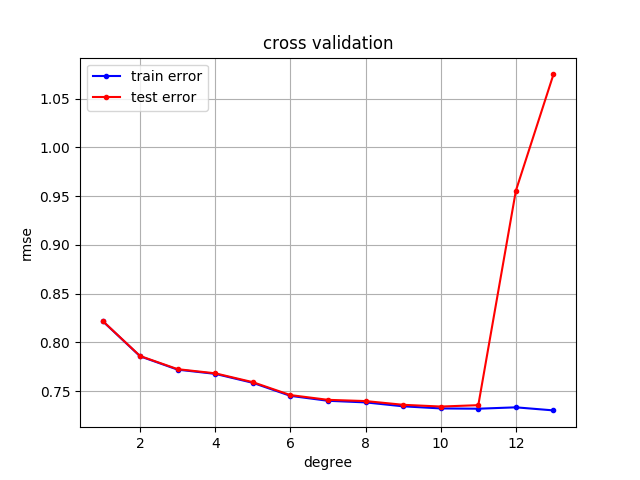
\includegraphics[width=\columnwidth]{cross_validation_leastsquares.png}
  \caption{RMSE for different degrees using least\_squares.}
  \vspace{-3mm}
  \label{fig:crossvalidationleastsquares}
\end{figure}




\begin{figure}[htbp]
	\centering
	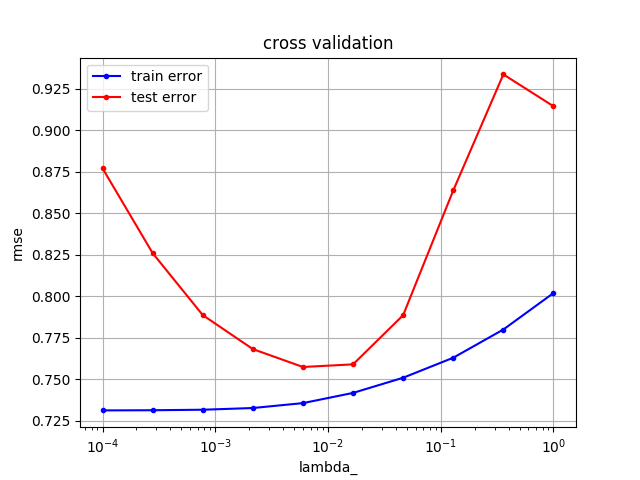
\includegraphics[width=\columnwidth]{cross_validation_ridge_degree_12.png}
	\caption{RMSE for different lambdas using ridge\_regression (degree 12).}
	\vspace{-3mm}
	\label{fig:crossvalidationridge}
\end{figure}
 %%%%pic to be added
 %%% find optimal lambda
 For the ridge\_regression a degree of!!!!range angeben?? 12 gave us the best result. Using cross validation we computed the \textit{RMSE} for different values of \textit{lambda\_} in order to optimize this hyperparameter. We find out, that a value of approximately 0.0059 gave the best result, which can be checked easily in Figure 2. When we choose this value too small, the test error gets much bigger, whereas the training error reduces. If \textit{lambda\_} is too big, both, the test and training error augment.\\

\section{Results}

\begin{table}[htbp]
	\centering
	\begin{tabular}[c]{|l||l|l|}
		\hline
		Methods&d&lambda\_\\
		\hline
		Least Square& 11 &-\\
		Least Square GD& 10 & -\\
		Least Square SGD & 10 &-\\		Ridge Regression&12&0.00599\\
		Logistic Regression & 10&-\\
		Reg. Logistic Regression&10&0.01\\
		\hline
	\end{tabular}
	\caption{Optimized hyperparameters computed\\ through 4-fold cross validation.}
	\label{tab:hyperpam}
\end{table}

After having optimized the hyperparameters for each model we want to see how the different models perform on the test data from CERN. We therefore submit each prediction on \textit{AICrowd} and see what result it gives us. In table 2 they can be easily compared.


\begin{table}[htbp]
	\centering
	\begin{tabular}[c]{|l||l|l|}
		\hline
		Methods&Accuracy&F1-Score\\
		\hline
		Least Square&0.821&0.723\\
		Least Square GD&0.566&0.012\\
		Least Square SGD&0.391&0.394\\		
		Ridge Regression&0.815&0.713\\
		Logistic Regression&0.673&0.12\\
		Reg. Logistic Regression&0.673&0.12\\
		\hline
	\end{tabular}
	\caption{Performances of our models submitted on AICrowd.}
	\label{tab:perform}
\end{table}

Least Squares performs best ending up with an accuracy of 0.821. For the \textit{degree} we chose the value 11. Ridgre regression performs good as well with an accurate choice of \textit{degree} 10 and \textit{lambda\_} 0.01. It gives an accuracy of 0.815.



All the other methods perform not as good as two mentioned above. Maybe this is because...´

\section{Discussion}

As mentioned before, least\_squares performs best concerning accuracy and F1-score. We did not take computational cost in account in order to compare the methods.
Is it actually surprising, that Least Squares Gradient performs that poor because in theory it would converge to the same optimum as Least Squares. Possible causes for this may be that we did not choose a good \textit{gamma} for the stepsize or we did not do enough iterations. 

For 


\section{Summary}




\bibliographystyle{IEEEtran}
\bibliography{literature}

\end{document}
